\documentclass{article}
\usepackage{arxiv}
\usepackage{iftex}
\ifPDFTeX\usepackage[utf8]{inputenc}\fi
\usepackage[T1]{fontenc}
\usepackage{amsmath,amssymb,booktabs,graphicx,microtype}
\usepackage[version=4]{mhchem}
\usepackage[numbers,sort&compress]{natbib}
\usepackage{url}
\usepackage{hyperref}
\usepackage{cleveref}
\usepackage{authblk}
\graphicspath{{figures/}}
% Generated from saved completed reports.
\newcommand{\BaselineCases}{15}
\newcommand{\FollowupCases}{64}
\newcommand{\TimeMin}{0.0043}
\newcommand{\TimeMax}{0.323}
\newcommand{\MeshMin}{2.06}
\newcommand{\MeshMax}{10.58}

\newcommand{\vect}[1]{\mathbf{#1}}
\newcommand{\units}[1]{\,\mathrm{#1}}
\title{Conservative CFD modelling of iodine deposition in thermal-gradient
columns: numerical verification and input sensitivity}
\renewcommand\Authfont{\bfseries}
\setlength{\affilsep}{0em}
\author[1]{Jan Kren}
\author[1]{Bojan Ni\v{c}eno}
\affil[1]{Paul Scherrer Institute, 5232 Villigen PSI, Switzerland}
\date{9 October 2026}
\renewcommand{\shorttitle}{Conservative CFD modelling of iodine deposition}
\renewcommand{\headeright}{Working manuscript}
\renewcommand{\undertitle}{Working manuscript for author review}
\hypersetup{colorlinks=true,linkcolor=blue,citecolor=blue,urlcolor=blue,
  pdftitle={Conservative CFD modelling of iodine deposition in thermal-gradient columns},
  pdfauthor={Jan Kren and Bojan Niceno}}
\begin{document}
\raggedbottom
\maketitle
\begin{abstract}
Interpreting iodine deposition in thermal-gradient columns requires a
consistent treatment of transport, gas speciation and exchange with
condensed wall inventories. We present a finite-volume model in OpenFOAM
for nine Pb--Bi--I gases in a frozen helium carrier, with element-conserving
gas equilibrium and shared wall reservoirs. Reversible iodide exchange
uses a Hertz--Knudsen--Schrage law coupled to the diffusive resistance
between a cell centre and its wall face. Published thermosublimatography
measurements supply three temperature profiles and deposition scans;
unreported source histories and flow-reference conditions are treated as
assumptions. Fifteen baseline and 64 follow-up simulations separate
numerical refinement from selected input sensitivities. For the 60 s
follow-up runs, the largest raw element-balance residue is
$8.85\times10^{-13}$ of supplied material. Halving the time step from
2 to 1 ms changes iodine deposition profiles by at most 0.323\%, whereas
refining from 18,432 to 41,472 cells changes them by 2.06--10.58\%; spatial
convergence remains unresolved. A $+29\units{kJ\,mol^{-1}}$ BiI gas Gibbs-energy
perturbation changes the refined steel-case BiI$_3$ share of deposited
iodide iodine from 94.57\% to 2.00\%, demonstrating strong conditional
thermochemical sensitivity. Two shifts derived from discrepancies between
the published silica temperature curve and its peak labels reduce
4--5 cm position errors to 0--1 cm, but do not establish a corrected
experimental coordinate system. The results support a conservative
computational method and an explicit assessment of uncertain inputs;
they do not establish independent predictive validation or reproduce
the three-hour experiment and subsequent cooling.
\end{abstract}
\keywords{Iodine deposition \and Thermosublimatography \and OpenFOAM
  \and Gas equilibrium \and Element conservation \and Input sensitivity}
\section{Introduction}
\label{sec:intro}
Iodine released from lead--bismuth eutectic (LBE) can be transported in
different chemical forms before depositing on cooler surfaces. The
chemical form matters because it determines both the gas-phase inventory
available for transport and the equilibrium pressure governing wall
exchange. Liu et al.\ \cite{Liu2025chemical} investigated this behaviour
by evaporating pure iodides and iodine-containing LBE into helium,
separating the products along a negative temperature gradient and
characterising the deposits. Their observations provide spatially
resolved evidence for PbI$_2$ and BiI$_3$ deposition, together with
potassium-containing deposits in some LBE experiments. Connecting such
measurements to a transport calculation requires more information than
a single deposition temperature: the temperature-coordinate mapping,
carrier flow, source history and gas composition all enter the predicted
distribution.

Lobresco et al.\ \cite{Lobresco2026assessment} compared temperature-based
and vapour-pressure-driven CFD deposition models. The former require
calibration of a deposition law; the latter connect deposition to
vapour-pressure information through interfacial kinetics. Their study
also motivates extending transport models to multiple chemical species
and thermodynamic equilibrium. A multispecies calculation introduces
an additional consistency requirement. Changes in chemical form must
preserve the transported elements, and different gas pathways leading
to the same condensed material must use one physical wall inventory.
An internally consistent implementation can nevertheless give uncertain
experimental predictions if the thermodynamic or source inputs are
poorly constrained.

The present work addresses these issues in the finite-volume framework
of OpenFOAM \cite{Weller1998tensorial}. Nine Pb--Bi--I gases are transported
in a prescribed helium carrier. Homogeneous gas equilibrium redistributes
the local elemental inventory, while separate interfacial channels
exchange material with immobile condensed wall reservoirs. The wall
flux includes both interfacial kinetic conductance and diffusion through
the distance from the neighbouring cell centre to the wall. This avoids
representing deposition by an arbitrarily chosen volumetric wall-layer
thickness. It does not remove spatial discretisation error.

Equilibrium-based reactive transport is also supported by general
thermodynamic packages such as GEM-Selektor and its GEMS3K kernel
\cite{Kulik2013gemselektor}. The software developed here contains a
GEMS3K interface, but the calculations reported in this paper use a
specialised ideal-gas element-potential solver with tabulated formation
constants. We therefore distinguish the thermodynamic formulation from
the particular numerical engine used in the reported simulations.
Condensed phases are handled through wall exchange rather than through
homogeneous cell equilibrium.

The study uses the published paper as its experimental input. No
author-supplied temperature files, release histories or mass-flow-controller
reference conditions are available. Instead of inferring a unique physical
source from deposition data, we report the consequences of two explicit
source constructions and selected variations in flow, diffusion,
interfacial accommodation and thermodynamic information. Separate
time-step and mesh studies identify which conclusions survive numerical
refinement. A temperature-coordinate discrepancy in the silica experiment
is examined as an input-consistency problem, with alternate mappings
defined from published quantities before comparing the resulting CFD
profiles.

The contribution is a documented conservative transport--equilibrium--wall
coupling and a completed numerical and input-sensitivity assessment.
The evidence comprises 15 baseline and 64 follow-up simulations of three
available experimental configurations. These are computational cases,
not independent experimental replicates. The scope is deliberately
restricted to the executed model: a fixed carrier and temperature field,
prescribed release, ideal-gas speciation, and wall deposits without aerosol
formation or surface-material-specific chemistry. Experimental comparisons
are conditional assessments of that model, rather than a claim of
independent predictive validation.

\section{Experimental basis and input reconstruction}
\label{sec:experiments}
\subsection{Available configurations}
The experimental columns of Liu et al.\ \cite{Liu2025chemical} were
1.25 m long, with an inner diameter of 4.8 mm for 316L stainless steel
and 5.0 mm for fused silica. A 15 mm sample boat was inserted into a
hot starting furnace, followed by a furnace providing a decreasing
temperature profile. Helium carried the evaporated material downstream.
The source was withdrawn after three hours; the furnaces and gas flow
were then turned off and the column cooled before deposit analysis.
Temperature measurements and radiotracer scans used 1 cm increments.

\Cref{tab:experiments} lists the three configurations for which both
temperature curves and iodine scans could be reconstructed. The
stand-alone BiI$_3$ experiment at 800\,$^\circ$C was considered in case
preparation but was not run, because its required axial temperature
profile was not available in the supplied figures. The missing case is
not assigned a surrogate profile or counted as an unsuccessful simulation.
\begin{table}[tb]
\centering
\caption{Published configurations used for the baseline matrix. Masses
refer to the initial sample, not to the amount released in a 60 s run.
All experimental evaporation periods were 10,800 s.}
\label{tab:experiments}
\begin{tabular}{llrrr}
\toprule
Identifier & Column & Diameter (mm) & Sample (mg) & He (mL/min) \\
\midrule
PbI2\_SS & Steel & 4.8 & 14.6 & 100 \\
LBE-I\_SS\_II & Steel & 4.8 & 346.0 & 45 \\
LBE-I\_SiO2\_I & Silica & 5.0 & 368.3 & 45 \\
\bottomrule
\end{tabular}
\end{table}

The two LBE samples had reported iodine mole fraction
$9.04\times10^{-4}$ and a 900\,$^\circ$C starting furnace. Their
reported deposited iodine amounts were 0.191 and 0.203 mg, respectively.
These deposited amounts constrain the prescribed mean iodine source in
the present cases; they are not direct measurements of a time-resolved
evaporation rate or an independent inlet-speciation measurement.

\subsection{Digitisation and coordinate assumptions}
Axial temperature curves and iodine histograms were digitised from the
published figures. Temperatures are linearly interpolated at cell centres
and wall faces; values beyond the plotted interval are held at the nearest
endpoint. The computational coordinate is identified with the plotted
coordinate. Its origin relative to the physical boat and furnace has not
been independently confirmed. \Cref{fig:temperature} displays the
reconstructed curves. These assumptions are retained in the original
baseline matrix and varied explicitly in the silica-coordinate study.

The recorded digitisation resolutions are approximately 1 mm in position,
4 K in temperature and 0.4 percentage points in histogram height. They
describe raster extraction, not the full experimental uncertainty. They
do not include coordinate registration, detector response, occluded curve
segments, temperature reproducibility or calibration. Likewise, the
uncertainties printed alongside experimental deposition temperatures
must not be interpreted as uncertainties on every digitised profile bin.
The reconstructed histogram sums are 99.17\%, 96.70\% and 102.24\%
for pure PbI$_2$, steel LBE and silica LBE. The primary comparison keeps
those values without silently renormalising them.

In the LBE scans, the paper assigns 6.6\% and 7.0\% of iodine to KI,
which is outside the Pb--Bi--I species set. The model profile is scaled
to the remaining 93.4\% or 93.0\%, while the measured histogram retains
all its published deposits. A second, explicitly conditional comparison
normalises both profiles over their common scanned range
(\cref{sec:comparison}). Neither comparison supplies the omitted
potassium chemistry.

\begin{figure}[tb]
\centering
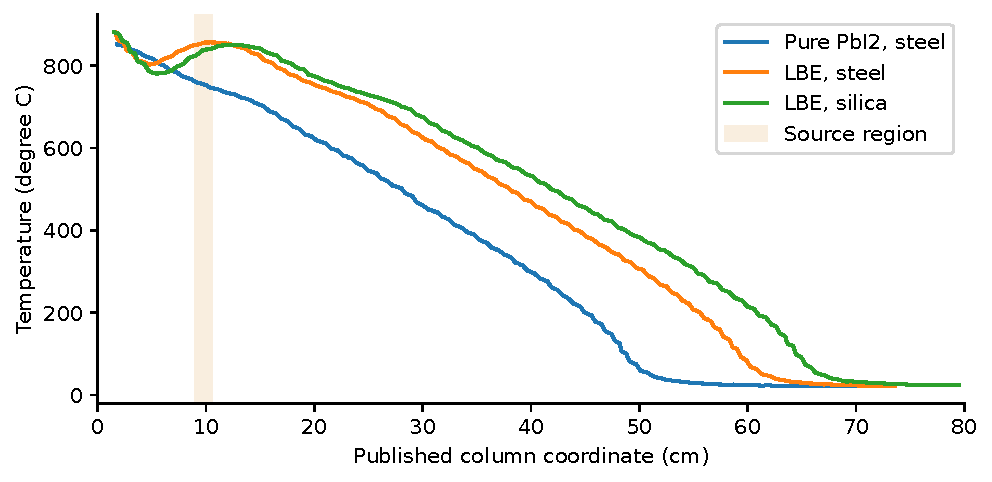
\includegraphics[width=.88\textwidth]{temperature_profiles.pdf}
\caption{Temperature curves digitised from Liu et al.\
\cite{Liu2025chemical}, with the assumed computational source interval.
Unplotted parts of the CFD domain use constant endpoint extensions.
The curves are experimental figure reconstructions, not temperature
fields predicted by a conjugate heat-transfer calculation.}
\label{fig:temperature}
\end{figure}

\subsection{Simulation duration and measurement protocol}
All source-driven cases run for 60 s while retaining a source rate based
on the 10,800 s experimental period. Thus they release $1/180$ of the
assumed three-hour inventory; the experimental inventory is not compressed
into a one-minute calculation. Continuous-source stationarity can inform
deposition rates and conditional shapes, but cumulative wall inventories
retain the initial filling transient. Four additional cases stop the
source and carrier flow at 60 s and continue to 80 s under the original
temperature profile. This probes residual-gas relaxation, not the
experimental cooling history.

%==============================================================================
\section{Mathematical model}
\label{sec:model}
%==============================================================================

%------------------------------------------------------------------------------
\subsection{Carrier-gas flow}
\label{sec:model:flow}
%------------------------------------------------------------------------------

The carrier gas is helium, treated as a laminar, steady, low-Mach-number ideal
gas ($\mathrm{Ma}\sim10^{-3}$) with density $\rho = pM_\mathrm{He}/(RT)$:
\begin{align}
  \nabla\cdot(\rho\vect{u}) &= 0, \\
  \nabla\cdot(\rho\vect{u}\vect{u}) &= -\nabla p + \nabla\cdot\boldsymbol{\tau},
  \qquad
  \boldsymbol{\tau} = \mu\left[\nabla\vect{u} + (\nabla\vect{u})^\mathsf{T}
    - \tfrac{2}{3}(\nabla\cdot\vect{u})\mathbf{I}\right], \\
  \nabla\cdot(\rho\vect{u}e) &= \nabla\cdot(\kappa\nabla T)
    - p\,\nabla\cdot\vect{u},
\end{align}
with $\mu(T)$ and $\kappa(T)$ from NIST helium data.  A Sutherland fit is
7--10\% low above \SI{1000}{K}; a power law
$\mu = \SI{1.9813e-5}{Pa.s}\,(T/\SI{300}{K})^{0.7027}$ stays within 0.6\% over
\SIrange{300}{1260}{K} (\cref{app:properties}).  At the inlet the
\emph{mass} flow rate is prescribed from the standard volumetric rate,
$\dot m = \rho_\mathrm{He}^\mathrm{STP}\dot V^\mathrm{STP}$ with
$\rho_\mathrm{He}^\mathrm{STP} = \SI{0.17848}{kg/m^3}$, so
\SIlist{5;106;540}{mL/min} correspond to
\SIlist{1.488e-8;3.155e-7;1.607e-6}{kg/s}.  The wall temperature is the
measured profile $T_w(x)$ for each flow rate.  Since the fully developed
gas--wall temperature difference is below \SI{1}{K} at \SI{106}{mL/min} and
about \SI{3}{K} at \SI{540}{mL/min} on the falling branch, the gas temperature
follows the wall closely.

\paragraph{Carrier-gas expansion.}  Between the \SI{\sim1070}{K} evaporation
zone and the \SI{300}{K} outlet the helium density changes by a factor of
about 3.5.  For a given mass flow, the local bulk velocity is therefore
$U_b(x) = (\dot V^\mathrm{STP}/A)\,T(x)/\SI{273.15}{K}$, which is 2.6--3.9 times
the standard-condition value in the deposition zone.  The T-Flows simulations of
\citet{Lobresco2026assessment} prescribe a uniform parabola with
$U_b = \dot V^\mathrm{STP}/A$ and unit density.  In that frame the transported
concentration is higher than the physical one by $T/\SI{273.15}{K}$, and the
residence time is longer by the same factor.
\todo{State this neutrally and confirm with the T-Flows authors before
submission (evidence: \texttt{Initialize\_Variables.f90}, \texttt{u\_max =
2*FLOW\_RATE/(pi*R\_PIPE**2)}; \texttt{Beginning\_Of\_Iteration.fpp},
\texttt{density = 1.0}; flat gas plateaus in their Fig.~9).}
For an equilibrium-controlled, reversible deposit the front sits where the
carrier that has swept past it, saturated at $p_v(T)$, could hold the whole
inventory $n_0$:
\begin{equation}
  p_v(\Tdep)\,\dot V(\Tdep)\,t = n_0 R\,\Tdep
  \quad\Longrightarrow\quad
  p_v(\Tdep) = \frac{n_0 R\,T_\mathrm{ref}}{\dot V^\mathrm{STP}\,t},
  \label{eq:equilibrium-front}
\end{equation}
where $T_\mathrm{ref} = \SI{273.15}{K}$ for the physical, expanding carrier.
With the non-expanding convention $T_\mathrm{ref}$ is replaced by $\Tdep$.
\todo{Preliminary estimate (1-D, digitized $p_v$ and $T_w$): the physical
kinematics give \SIlist{807;729;678}{K} for T106\_6/60/300 against measured
\SIlist{814;723;667}{K} (RMS \SI{8}{K}); the non-expanding convention
reproduces the published vapor-pressure-model values
(\SIlist{841;760;701}{K}, RMS error \SI{33}{K}).  Confirm with the full CFD --
potentially a headline result.}

\decide{Frozen carrier vs.\ two-way coupling.  The flow is solved once and
frozen.  During sample evaporation the \ce{PbI2} mole fraction reaches 0.2--3\%
(12\% for T5\_60), but its mass ratio to He reaches 1--16 because
$M_{\ce{PbI2}}/M_\mathrm{He}=115$.  Either justify the passive-scalar
assumption quantitatively (and exclude T5\_60) or solve continuity with the
mixture density.}

%------------------------------------------------------------------------------
\subsection{Species transport}
\label{sec:model:species}
%------------------------------------------------------------------------------

Each gaseous species $i$ is transported as $Y_i$, the mass of species $i$ per
unit mass of carrier.  With the frozen He density this is a mass ratio, not
bounded by one:
\begin{equation}
  \frac{\partial(\rho Y_i)}{\partial t} + \nabla\cdot(\rho\vect{u}Y_i)
  = \nabla\cdot\left(\rho D_i\nabla Y_i\right)
    - \nabla\cdot\vect{j}_i^{T} + \dot s_i .
  \label{eq:species}
\end{equation}
Here $\dot s_i$ [\si{kg.m^{-3}.s^{-1}}] is the phase-change source and
$\vect{j}_i^{T}$ an optional thermal-diffusion (Soret) flux.  For a heavy
trace species in a light carrier
\begin{equation}
  \vect{j}_i^{T} = -\rho D_i\,\alpha_{T,i}\,Y_i\,\nabla\ln T ,
  \label{eq:soret}
\end{equation}
with $\alpha_{T,i}>0$ driving the heavy species towards colder regions.
Fick's law is written for the mass (mole) fraction, which is the correct form
for a non-isothermal ideal gas.  With a constant-density carrier, as in
\citet{Lobresco2026assessment}, it reduces to $-D\nabla c$.
\decide{Include \cref{eq:soret}?  It needs $\alpha_T$ for \ce{PbI2}--He
(Chapman--Enskog).  The axial gradient in the deposition zone is
\SIrange{1200}{1500}{K/m}; the radial gradient is small (thermal P\'eclet
number $\approx0.7$).  A first estimate (literature review, Sect.~10) gives a radial Soret drift of
0.2--1\% of the wall mass-transfer coefficient: likely negligible; keep as a
sensitivity case only.}

\paragraph{Binary diffusivity.}  $D_i$ follows from Chapman--Enskog theory
\begin{equation}
  D_{i,\mathrm{He}}\,[\si{cm^2/s}] = \frac{1.86\times10^{-3}\,T^{3/2}}
       {p\,\sigma_{i,\mathrm{He}}^2\,\Omega^{(1,1)*}(T^*)}
       \sqrt{\frac{1}{M_i}+\frac{1}{M_\mathrm{He}}},
  \qquad T^* = \frac{k_BT}{\varepsilon_{i,\mathrm{He}}},
  \label{eq:diffusivity}
\end{equation}
with $p$ in atm, $M$ in g/mol and $\sigma$ in \AA.  The \ce{PbI2}
Lennard-Jones parameters come from its computed static polarizability
(116.3~a.u.\ $=\SI{17.23}{\angstrom^3}$) through the Brandt (1956)
correlation with $N=16$ electrons: $\sigma_{\ce{PbI2}} = \SI{5.966}{\angstrom}$
and $\varepsilon/k_B = \SI{495.9}{K}$.  With He from tables (\SI{2.551}{\angstrom},
\SI{10.2}{K}) the mixing rules give $\sigma_{12}=\SI{4.2585}{\angstrom}$ and
$\varepsilon_{12}/k_B=\SI{71.118}{K}$.  These values are not stated in
\citet{Lobresco2026assessment} and are needed to reproduce their Fig.~3.
\decide{Two known biases.  (i) The five-coefficient $\Omega$ fit of
\citet{Lobresco2026assessment} lies 0.5--8.7\% below Neufeld et al.\ (1972) for
$T^*=4$--$15$, so $D$ is 8--9.5\% too high at \SIrange{666}{1100}{K}.
(ii) The valence-electron count of \ce{PbI2} is 18, not 16; using 18 lowers
$D$ by 2.4--3.1\%.  The Brandt route itself is uncertain by more than 10\% for
heavy halides.  Proposal: keep the published fit in the code-to-code
comparison, use Neufeld in the physical model, and propagate a $\pm15\%$
uncertainty in $D$.}

%------------------------------------------------------------------------------
\subsection{Condensed phases and gas--solid phase change}
\label{sec:model:phasechange}
%------------------------------------------------------------------------------

Condensed material is immobile.  It is held in two reservoirs: the
evaporating sample, as a volumetric density $C_{s}$ [\si{kg/m^3}] in the sample
cells, and the wall deposit, as a surface density $m''_{w}$ [\si{kg/m^2}] on
each wall face.  Phase change is written as a net \emph{evaporation} mass flux
$\dot m''_i$ [\si{kg.m^{-2}.s^{-1}}] across an interface of area $A$:
\begin{equation}
  \dot s_i\big|_\mathrm{cell} = \frac{1}{V}\sum_{f\in\mathrm{wall}}
      \dot m''_{i,f}A_f ,
  \qquad
  \frac{\partial m''_{w,i}}{\partial t} = -\dot m''_{i} .
  \label{eq:wallflux}
\end{equation}
Gas plus condensed mass is therefore conserved exactly by construction, and the
deposit per unit wall area does not depend on the first-cell thickness.  On the
mesh of \citet{Lobresco2026assessment} (first cell $57.46\,\mu\mathrm{m}$),
exactly one cell layer lies entirely within their \SI{0.1}{mm} interaction
layer, with $A_I/V_I = \SI{17682}{m^{-1}}$.  A cell-centre distance test would
select two layers and halve $A_I/V_I$.

\paragraph{Temperature-based model.}  The calibrated model of
\citet{Lobresco2026assessment} (their Eq.~5) is a volumetric sink in the wall
layer.  In flux form it becomes
\begin{equation}
  \dot m''_i = -\,v_d\left[1-e^{-k(\Tdep-T)}\right]^{+}\rho Y_i ,
  \qquad v_d = A\,\frac{V_I}{A_I} ,
  \label{eq:tempmodel}
\end{equation}
with $[\cdot]^{+}=\max(\cdot,0)$.  For $A=\SI{220}{s^{-1}}$ on their mesh,
$v_d = \SI{1.24}{cm/s}$.  Wall uptake is thus kinetics-limited: $v_d$ is about
0.1 of the laminar mass-transfer coefficient $k_m = 3.66\,D/d\approx\SI{0.1}{m/s}$.
The calibrated $A$ therefore belongs to that mesh (it scales with $1/h_1$);
$v_d$ is the mesh-independent parameter.  The calibration also assumed the
non-expanding carrier: keeping the same decay length with physical velocities
requires $v_d$ to be larger by about $T/\SI{273.15}{K}$.
\todo{Recalibrate against the Liu reference histogram in physical kinematics.
The $\Tdep$ correlation of \citet{Liu2025chemical} must be obtained; it is not
in either paper's text we have.}

\paragraph{Hertz--Knudsen--Schrage model.}  The net evaporation flux is
\begin{equation}
  \dot m''_i = C_e\,\frac{2\sigma_a}{2-\sigma_a}
     \sqrt{\frac{M_i}{2\pi RT}}\,\bigl[p_{v,i}(T) - p_i\bigr],
  \qquad p_i = \frac{\rho Y_i RT}{M_i},
  \label{eq:hks}
\end{equation}
in SI units ($M_i$ in kg/mol, pressures in Pa).  Evaporation
($\dot m''_i>0$) is allowed only where condensate exists, and deposition only
at walls \citep[cf.\ Fig.~7 in][]{Lobresco2026assessment}.  With $\sigma_a=1$
the kinetic velocity $\frac{2\sigma_a}{2-\sigma_a}\sqrt{RT/(2\pi M)}$ is
\SI{\sim90}{m/s} at \SI{700}{K}.  That is about $10^3$ times the diffusive
supply $k_m$, so in consistent units wall deposition is
\emph{transport-limited}: the near-wall gas sits at $p_v(T_w)$, and the flux
hardly depends on $C_e$.  In the wall layer the implied relaxation rate
$\sim\SI{1.6e6}{s^{-1}}$ must be treated implicitly.
\decide{The reference T-Flows implementation evaluates $p_v$ and $p_i$ in bar
and $M$ in g/mol inside the SI prefactor.  It also multiplies $A_I/V_I$ by
200 in the wall layer and uses $5\times2/R_\mathrm{sample}$ at the sample
(\texttt{LESTO\_HKS/User\_Mod/Source.fpp}, \texttt{Types.f90}).  A 1-D fit to
their Fig.~11 needs a rate factor of about $10^{-5}$ relative to SI.  If this
is confirmed, their conclusion that condensation kinetics are "slower than in
the experiment" (hence $C_e>1$) is a units effect.  Must be discussed with
F.~Lobresco and B.~Ni\v{c}eno before it enters the paper.}

%------------------------------------------------------------------------------
\subsection{Chemical equilibrium with GEMS3K}
\label{sec:model:gems}
%------------------------------------------------------------------------------

For multi-species chemistry the vapor pressures $p_{v,i}(T)$ are replaced by
local equilibrium from the Gibbs energy minimization kernel GEMS3K
\citep{Kulik2013gemselektor,Wagner2012gemselektor}.  In each interfacial (and sample) cell the
bulk elemental composition $\vect{b}$ of gas plus adjacent condensate (Pb, Bi,
I, He \decide{+ O?}) is assembled from the transported species and the
deposit, with the carrier amount $n_\mathrm{He} = pV/(RT)$.  GEMS3K then solves
\begin{equation}
  \min_{\vect{n}\ge0}\; G(\vect{n};T,p) \quad\text{s.t.}\quad
  \mathbf{A}\vect{n} = \vect{b},
\end{equation}
which gives the equilibrium amounts $\vect{n}^\mathrm{eq}$ of all gaseous
species (\ce{PbI2}, \ce{PbI}, \ce{Pb}, \ce{I}, \ce{I2}, \ce{BiI3}, \ce{BiI},
\ce{Bi}, \ldots) and condensed phases (\ce{PbI2}(s,l), \ce{BiI3}(s),
\ldots).  The equilibrium partial pressures $p_i^\mathrm{eq}$ over the local
condensed assemblage replace $p_{v,i}(T)$ in \cref{eq:hks}; for pure \ce{PbI2}
this reduces to the two-phase vapor pressure.  This coupling requires the
physical (expanding) carrier, because only there are the concentrations
physical.
Open, redistributable data suffice for Pb--I--He: the Gurvich (1991)
evaluation as distributed with NASA CEA (Apache-2.0), cross-checked against
NIST-JANAF, covers \ce{He}, \ce{I}, \ce{I2}, \ce{Pb}, \ce{PbI}, \ce{PbI2}(g)
and \ce{PbI2}(cr,l), \ce{Pb}(cr,l).  With these data a GEMS3K system generated
without GEM-Selektor reproduces the speciation of Fig.~4 of
\citet{Lobresco2026assessment} and returns $p_{\ce{PbI2}}$ over the stable
condensed phase to $|\Delta\log_{10}p| < 10^{-4}$ of the direct evaluation
(\SIrange{500}{1100}{K}).
\todo{Two findings to state carefully: (i) the $p_v(T)$ of their Fig.~6 is
the gas--\emph{solid} curve extrapolated through the melting point
($T_m=\SI{683}{K}$); over the stable liquid, $p_v$ is lower by a factor of 2.1
at \SI{823}{K}, 4 at \SI{1000}{K} and $\sim$7 at \SI{1173}{K}, i.e.\ in the
evaporation zone.  (ii) JANAF \ce{PbI4}(g) is spurious and must be excluded
(it disproportionates \ce{PbI2} over condensed Pb); Gurvich \ce{PbI4} is
harmless.  Bi--I data exist only in HERACLES (Barin-derived, GPL-3; no
\ce{BiI3}(l), defective Pb(g) record) -- provenance to confirm with PSI.}
\decide{Coupling: (a) HKS driven by GEMS $p_i^\mathrm{eq}$ (recommended;
reduces to the published model); (b) instantaneous local equilibrium
(operator-split); (c) relaxation towards $\vect{n}^\mathrm{eq}$.  Thermodynamic
database: HSC MainDB (commercial) vs.\ an open database -- licensing for
distributing GEMS3K input files.}

%------------------------------------------------------------------------------
\subsection{Acceleration of the equilibrium calls}
\label{sec:model:surrogate}
%------------------------------------------------------------------------------

Measured cost with the open-data Pb--I--He system, called from an OpenFOAM
application through a plain-C bridge: $60\,\mu$s per warm-started
equilibrium (3.9 iterations on average, no failures in $5\times10^4$ calls
along a \SIrange{1100}{400}{K} wall profile).  At $\Delta t=\SI{1}{ms}$ a
\SI{60}{s} run needs $9\times10^8$ calls if restricted to the 15\,264 wall
cells, i.e.\ about 15~CPU-hours -- the same as the transport itself.
Direct coupling in interfacial cells is therefore affordable; tabulation
\citep{Pope1997computationally} or learning-based surrogates
\citep{Leal2020accelerating,Prasianakis2020neural} become necessary only for
calls in every cell or for non-ideal multi-component phases.
\todo{Re-measure for the Pb--Bi--I system.}
\decide{Include surrogates in this paper or defer?}

\section{Numerical implementation and study design}
\label{sec:numerics}
\subsection{Geometry and carrier preparation}
A structured axisymmetric 5$^\circ$ wedge represents the 1.25 m column
(\cref{fig:geometry}). The steel and silica radii are 2.4 and 2.5 mm,
respectively. The baseline mesh has $384\times48\times1=18{,}432$
cells. Coarse and fine meshes have $256\times32\times1=8{,}192$ and
$576\times72\times1=41{,}472$ cells, refining axial and radial spacing
by a factor of 1.5 between successive levels. The source spans
$x=0.09$--0.105 m and the radial interval $r=0.25R$--$0.75R$.
Its position and selection are computational assumptions; the physical
boat is omitted from the carrier geometry. Full-column source and inlet
rates are multiplied by $5/360=1/72$ for the wedge.

\begin{figure}[tb]
\centering
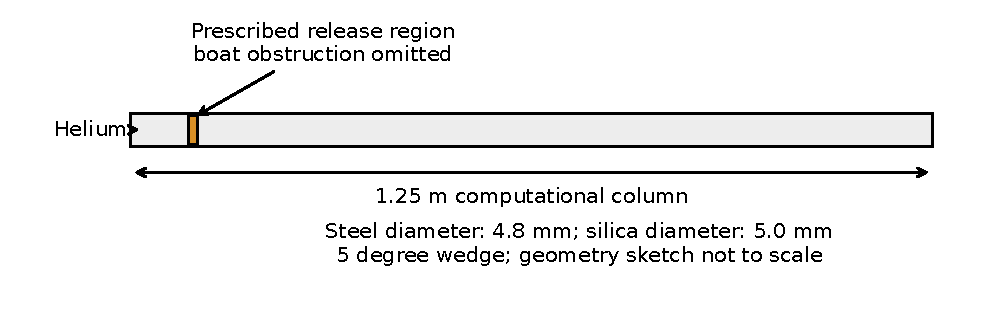
\includegraphics[width=.94\textwidth]{experiment_schematic.pdf}
\caption{Computational geometry and prescribed source region. The source
is distributed in selected cells; the sketch does not represent a
resolved boat surface. Tube length and material-specific diameters are
retained, and the 5$^\circ$ wedge supplies the axisymmetric reduction.}
\label{fig:geometry}
\end{figure}

The inlet flow rates are converted to helium mass flow assuming a
controller reference of 298.15 K and 101,325 Pa. Full-column rates are
$2.727\times10^{-7}\units{kg\,s^{-1}}$ at 100 mL/min and
$1.227\times10^{-7}\units{kg\,s^{-1}}$ at 45 mL/min. The reference
conditions are not specified by the supplied paper. A separate study
uses 273.15 K at the same reference pressure. Helium uses the perfect-gas
law, constant heat capacity and Sutherland viscosity
(\cref{app:properties}). Steady laminar carriers are prepared with
\texttt{rhoSimpleFoam}; the reconstructed temperature profile remains
prescribed.

The converged face mass flux is retained instead of reconstructing it
from interpolated velocity. At these low mass flows, residual discrete
divergence is removed by a zero-initialised potential correction before
species transport. Carrier preparation rejects an original cell or global
flux defect exceeding $10^{-6}$ of inlet flow, or a flux/velocity
correction exceeding $10^{-5}$ of the corresponding scale. After
correction, inlet, global and cell continuity and impermeable-boundary
leakage are audited against $10^{-12}$ of inlet flow. This procedure
makes the frozen transport field discretely conservative; it is not a
new physical flow model or evidence of convergence of the velocity field.

\subsection{Discretisation and coupling}
The transient species equations use implicit Euler time integration,
first-order upwind advection and corrected Gauss linear diffusion. All
nine transported gases use the same advection scheme. The baseline time
step is 2 ms. Wall exchange is assembled implicitly with nonnegative
source and sink coefficients and shared inventory bounds. Configured
species correctors and active-bound guards reconcile the final gas
solution with the realised wall transfer. Gas re-speciation then
redistributes species under the local element constraints. This sequence
is first order in time; a conservative equilibrium projection alone
does not eliminate splitting or transport error.

The baseline configuration requests three species correctors with a
$10^{-16}$ tolerance and up to eight bound guards with a $10^{-13}$
guard tolerance. These are stopping settings, not guarantees that every
outer wall-regime iteration attains the requested tolerance. The final
transport defect, bound status and material ledger must be examined
independently (\cref{sec:conservation}). Additional short corrector
replays isolate late-time iteration sensitivity but do not establish
full-run iteration independence.

The baseline diffusivity is $D_i=10^{-4}\units{m^2\,s^{-1}}$ for every
gas. Three transport alternatives halve or double this value for all
gases, or replace only the PbI$_2$ coefficient by a temperature- and
pressure-dependent PbI$_2$--He estimate. The latter's collision
parameters are estimates, not independently measured binary transport
data. Accommodation variations change the two reversible iodide pairs
to $\alpha=0.1$ or 0.01, retaining the baseline metal-channel coefficients.

\subsection{Completed case matrix}
The 15 baseline cases comprise Q1 for each available configuration and
Q2 for the two LBE columns, at
$\beta\in\{0.001,0.01,0.1\}$ with two thermodynamic branches. The
second branch adds a constant 29 kJ/mol to BiI(g)'s standard Gibbs energy;
it is a sensitivity surrogate, not a second experimentally qualified
dataset. All completed calculations use the same solver executable,
identified by its SHA-256 in the saved reports.

\Cref{tab:study} describes the 64 follow-up cases. Mesh and time-step
checks cover pure PbI$_2$ and three steel Q2 cases: baseline
thermodynamics at 0.1\% and 1\% metal saturation and shifted BiI
thermodynamics at 1\%. Physical transport, accommodation, source-position
and flow-reference variations cover pure PbI$_2$, those two baseline
steel Q2 cases, and silica Q2 at 0.1\%. Extra source-loading cases use
both columns and both thermodynamic branches. Temperature-coordinate
variants use silica Q1 and silica Q2 at 0.1\%. This is a structured
set of conditional comparisons, not a factorial uncertainty study.
\begin{table}[tb]
\centering
\caption{Completed follow-up matrix. The baseline cases are additional
references. Numerical comparisons use one changed resolution at a time;
flow-stop cases continue a 60 s baseline to 80 s.}
\label{tab:study}
\small\begin{tabular}{lrl}
\toprule
Study & Cases & Variation \\
\midrule
Mesh and time step & 12 & Three grids; 2 and 1 ms \\
Gas diffusion & 12 & $D/2$, $2D$, PbI2--He correlation \\
Iodide accommodation & 8 & $\alpha=0.1$, 0.01 \\
Source position & 8 & $\Delta x_s=\pm1.5$ cm \\
Q2 metal loading & 12 & $\beta=0.002$, 0.003162, 0.005623 \\
Flow reference & 4 & 273.15 versus 298.15 K \\
Silica temperature coordinates & 4 & $\Delta x_T=-4.10$, $-4.65$ cm \\
Flow-stop relaxation & 4 & 60--80 s; fixed temperature \\
\bottomrule
\end{tabular}

\end{table}

The source-position alternatives move the release region by
$\pm1.5\units{cm}$ without adding a boat obstruction. Flow-stop cases
restart the saved 60 s fields, remove injection, set carrier flow to
zero and impose zero normal species flux at both ends. The original
nonuniform temperature profile stays fixed. Their comparisons therefore
measure redistribution of residual gas during a 20 s fixed-temperature
flow stop, not a clean-helium purge or a full cooling calculation.

%==============================================================================
\section{Verification}
\label{sec:verification}
%==============================================================================

\todo{Planned verification hierarchy:}
\begin{enumerate}
  \item \textbf{Conservation.}  Closed box ($\phi=0$, uniform sink rate
        $\lambda$): $\int\rho Y\,\mathrm{d}V$ must decay as
        $(1+\lambda\Delta t)^{-n}$ and gas plus deposit must stay constant to
        round-off.  Open tube: $\int\dot m_\mathrm{in}\mathrm{d}t =
        M_\mathrm{gas} + M_\mathrm{deposit} + \int\dot m_\mathrm{out}\mathrm{d}t$
        for both deposition models and for the GEMS coupling.
  \item \textbf{Analytical solution.}  Isothermal, fully developed laminar
        flow with a first-order wall sink (Graetz problem with a Robin
        condition): axial decay of the bulk value and of the wall flux against
        the eigenfunction solution \todo{cite}; grid convergence (GCI).
  \item \textbf{Code-to-code against T-Flows (``paper mode'').}  Constant
        density and a uniform parabola with $U_b=\dot V^\mathrm{STP}/A$ (inlet
        flux rescaled for the 0.51\% facet-area deficit), the digitized or
        measured $T_w(x)$, NIST He, the published $\Omega$ fit, the same sample
        source, $A$, $k$, $\Tdep$, $\sigma_a$, $C_e$ and $p_v(T)$ -- and, for
        HKS, the unit convention of the reference code.  In this mode
        \cref{eq:species} reduces term by term to Eq.~(1) of
        \citet{Lobresco2026assessment}.  Targets: the gas line density
        $n'\,t_\mathrm{ev} = \SI{3.38e-4}{mol.s/m}$ (their Fig.~9), the solid
        independent of $t_\mathrm{ev}$, the Fig.~11 profiles and the Fig.~12
        front positions.
        \decide{Pin the reference parameter set.  The paper and the T-Flows
        branches differ ($A_I/V_I$ multipliers $\times200$/$\times5$, $A$,
        $k$, one or two wall layers), and Figs.~9 and 10 are not mutually
        consistent with $A=\SI{220}{s^{-1}}$, $k=\SI{8e-3}{K^{-1}}$,
        $\Tdep=\SI{680}{K}$.}
  \item \textbf{Effect of each modeling change} (``physical mode''), one at a
        time: expanding carrier; SI-consistent HKS; Neufeld collision integral;
        mesh-independent wall flux; Soret term.
\end{enumerate}

%==============================================================================
\section{Validation: \ce{PbI2} thermosublimatography}
\label{sec:validation}
%==============================================================================

\todo{Simulate the five experiments of \cref{tab:experiments} with both
deposition models in physical mode and compare deposition profiles and
deposition temperatures.  As in \citet{Lobresco2026assessment}, $\Tdep$ is the
wall temperature at the first axial position where the deposit exceeds 1\% of
its peak (linear interpolation).  Simulated profiles are also rebinned to the
\SI{1}{cm} bins of the $\gamma$-scan.}

\begin{table}[h]
  \centering
  \caption{Deposition temperatures [K]: experiment and T-Flows models from
    \citet{Lobresco2026assessment} (Table~2), and the present work.}
  \label{tab:tdep}
  \begin{tabular}{lrrrrr}
    \toprule
    Case & Experiment & T-based & VP-based & This work (HKS) &
      This work (GEMS) \\
    \midrule
    T106\_6   & 814 & 775 & 841 & -- & -- \\
    T106\_60  & 723 & 713 & 760 & -- & -- \\
    T106\_300 & 667 & 666 & 701 & -- & -- \\
    T5\_60    & 847 & 787 & 797 & -- & -- \\
    T540\_60  & 700 & 670 & 685 & -- & -- \\
    \bottomrule
  \end{tabular}
\end{table}

\paragraph{What the targets test.}  The temperature-based column equals the
input $\Tdep^\mathrm{calc}$ of \cref{tab:experiments} to within $\pm\SI{1}{K}$,
so it only checks that the onset follows the imposed $\Tdep$.  The
vapor-pressure column is set by equilibrium thermochromatography
(\cref{eq:equilibrium-front}) and is insensitive to the kinetic parameters.
Kinetics show only in the peak height, width and tail of the profiles.
Acceptance criteria are therefore profile-based: onset position, peak
position and height, and integral $\approx n_0$.  $\Tdep$ agreement is only
testable to the accuracy of the wall-temperature data ($\pm\SI{15}{K}$
thermocouples; a \SI{1}{cm} shift corresponds to \SIrange{12}{15}{K} at
\SIrange{1200}{1500}{K/m}).
\todo{T5\_60: the published HKS value comes from an upstream back-diffusion
deposit on the steep rising branch; evaluate on the main deposit instead.}

\todo{Sensitivity: $\sigma_a$/$C_e$, wall temperature ($\pm\SI{15}{K}$), flow
rate ($\pm5\%$), $D$ ($\pm15\%$), Soret term, $p_v$ source (GEMS vs
Binnewies--Milke: \SIrange{15}{25}{K} in $\Tdep$).}

\section{Input sensitivity and interpretation}
\label{sec:sensitivity}
\subsection{Source loading and thermodynamic information}
The Q2 cases expose a sensitivity hidden by prescribing the iodide
split. \Cref{fig:thermo} shows the BiI$_3$ iodine fraction
\begin{equation}
 f_{\rm BiI_3}=
 \frac{3N^{\rm wall}_{\rm BiI_3}}
 {2N^{\rm wall}_{\rm PbI_2}+3N^{\rm wall}_{\rm BiI_3}}.
 \label{eq:split}
\end{equation}
This includes only iodine in the two modelled deposited iodides.
It is distinct from the BiI$_3$ fraction of all experimental iodine,
which also contains KI. Additional metal-saturation cases fill selected
points between the original 0.1\% and 1\% branches; line segments
connect computed points and are not a fitted release law.

At 1\% metal saturation on the fine steel mesh, the baseline
thermodynamics gives $f_{\rm BiI_3}=94.57\%$. Raising the BiI(g)
standard Gibbs energy by 29 kJ/mol gives 2.00\% with the same numerical
resolution. The large difference survives refinement, demonstrating
conditional thermodynamic sensitivity rather than numerical noise.
The perturbation is applied consistently to formation and reactive-wall
constants. A constant Gibbs-energy shift scales the formation constant
by $\exp[-29{,}000/(RT)]$, approximately 0.051 at 1173 K and
0.00093 at 500 K. It is a substantial surrogate perturbation, not an
independently measured correction to BiI thermodynamics.

Source loading also matters. With baseline thermodynamics the steel
BiI$_3$ share at 0.2\%, 0.316\% and 0.562\% metal saturation is
52.50\%, 70.58\% and 94.56\%; the shifted branch gives 47.66\%,
37.43\% and 15.88\%. The low-loading trend is not universally
monotonic. The original steel 0.1\% baseline branch gives 56.47\%
and an 81.10\% scan overlap, making it a useful diagnostic comparison,
but not an identified physical saturation. The published deposits alone
cannot uniquely distinguish source loading, thermodynamic information
and omitted chemistry. Choosing a branch because it best matches one
scan would introduce calibration and require independent validation.

\begin{figure}[tb]
\centering
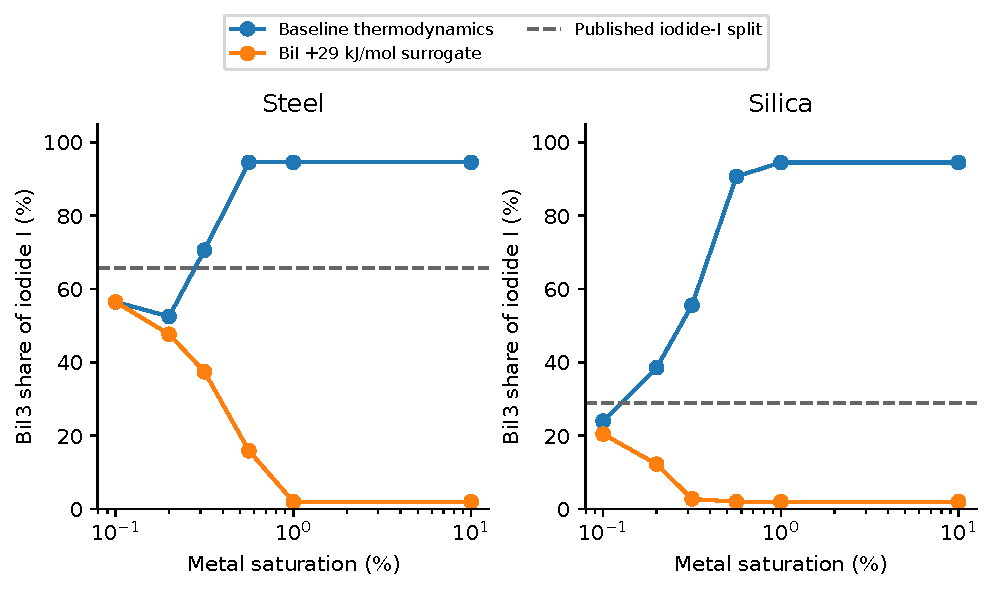
\includegraphics[width=.96\textwidth]{source_thermodynamics.pdf}
\caption{Conditional source-loading and BiI thermodynamic sensitivity
for steel and silica LBE. Symbols denote completed Q2 cases; segments
only connect those points. Dashed grey lines show the published
BiI$_3$ share after excluding KI \cite{Liu2025chemical}.
The $+29$ kJ/mol branch is a surrogate perturbation, not a second
qualified thermodynamic dataset.}
\label{fig:thermo}
\end{figure}

\subsection{Silica temperature-coordinate discrepancy}
\label{sec:silica}
The published silica scan places PbI$_2$ and BiI$_3$ maxima at 51 and
59 cm, labelled 306$\pm$24 and 127$\pm$39\,$^\circ$C. At those
coordinates, the digitised temperature curve gives approximately 369
and 235\,$^\circ$C: differences of 63 and 108 K. On that same
curve, 306 and 127\,$^\circ$C occur at 55.096 and 63.653 cm.
The discrepancy exceeds the nominal raster temperature resolution and
suggests a temperature-coordinate consistency problem in the supplied
inputs. It does not identify which measurement, annotation or registration
requires correction.

Two diagnostic mappings shift only the silica temperature curve upstream
by 4.096 or 4.653 cm, aligning one of those curve crossings with the
corresponding labelled position. Equivalently,
$T_\delta(x)=T_0(x+\delta)$ for $\delta>0$, with
$\Delta x_T=-\delta$. The gamma scan remains fixed. These shifts are
derived from the published curve and labels, not optimised against the
CFD profiles. All original unshifted results are retained.

\Cref{tab:alignment,fig:alignment} shows that the shifts move Q1 maxima
from 56/63 cm to 52/59 or 51/58 cm and improve normalised overlap from
7.20\% to 75.29\% or 81.00\%. The low-loading Q2 variants place
both maxima at 51/59 cm, with overlaps 79.16\% and 83.33\%.
This explains why a plausible coordinate change has a larger effect
than the tested source-position or time-step changes. It does not
confirm either shift as the experimental truth. The two shifts also
produce different peak temperatures and cannot simultaneously reconcile
both original temperature labels by a uniquely established mapping.
\begin{table}[tb]
\centering
\caption{Silica temperature-coordinate hypotheses. Shifts and peak
positions are in cm; raw L1 is in percentage points and overlap in
percent. Q2 uses baseline thermodynamics and 0.1\% metal saturation.
Every row uses the same fixed experimental scan.}
\label{tab:alignment}
\small\begin{tabular}{lrrrrr}
\toprule
Source & $\Delta x_T$ & $x_{\rm PbI_2}$ & $x_{\rm BiI_3}$ & Raw L1 & Overlap \\
\midrule
Q1 & 0.00 & 56 & 63 & 181.84 & 7.20 \\
Q1 & -4.10 & 52 & 59 & 46.28 & 75.29 \\
Q1 & -4.65 & 51 & 58 & 37.05 & 81.00 \\
Q2 & 0.00 & 56 & 63 & 181.84 & 7.20 \\
Q2 & -4.10 & 51 & 59 & 39.40 & 79.16 \\
Q2 & -4.65 & 51 & 59 & 34.31 & 83.33 \\
\bottomrule
\end{tabular}

\end{table}
\begin{figure}[tb]
\centering
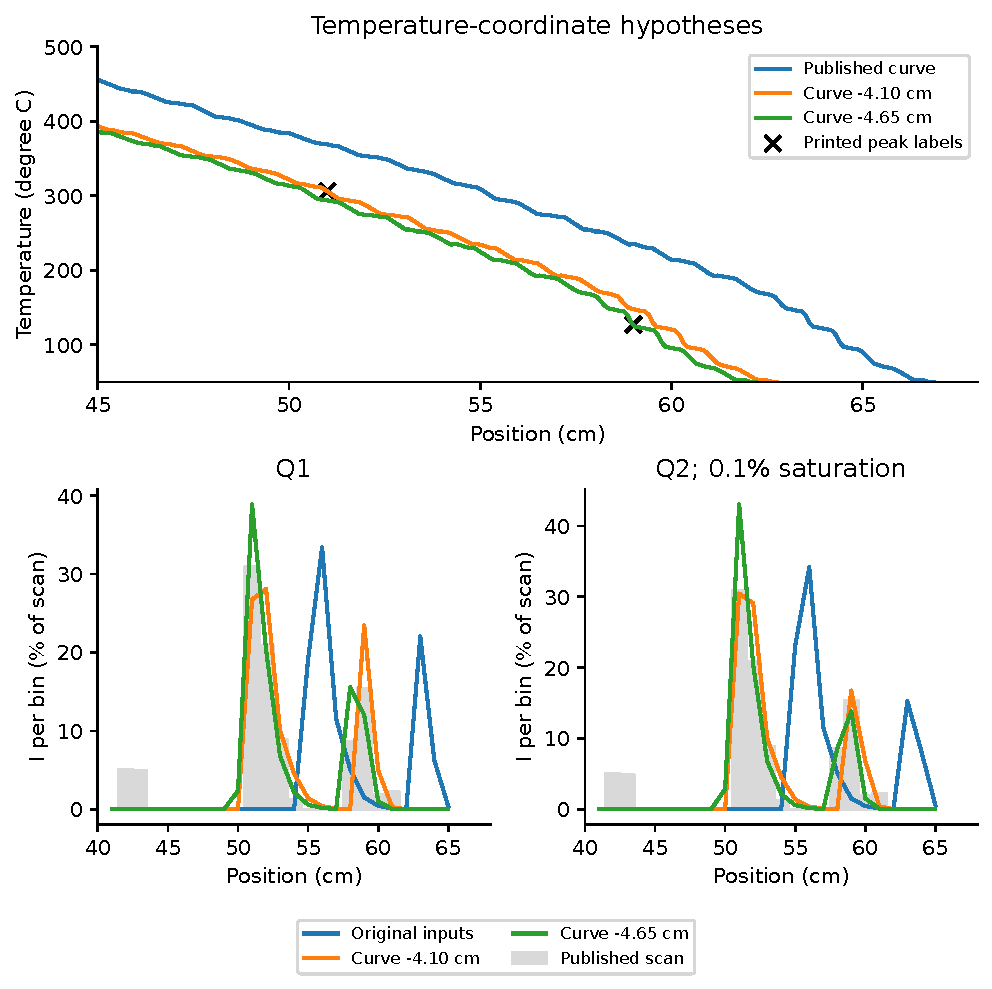
\includegraphics[width=\textwidth]{silica_alignment.pdf}
\caption{Input-derived silica mappings and their consequences.
Top: the original reconstructed temperature curve, two shifts and
printed peak labels. Bottom: common-scan-normalised iodine
profiles for Q1 and low-loading Q2. Improved agreement is conditional
on an unconfirmed coordinate hypothesis. Published data are adapted
from Liu et al.\ \cite{Liu2025chemical}.}
\label{fig:alignment}
\end{figure}

The shifted low-loading Q2 cases retain a BiI$_3$ share near 23.97\%,
about five percentage points below the published iodide-only split.
Correct peak positions therefore do not ensure the correct partition.
Resolving the discrepancy requires the original thermocouple profile
and its coordinate registration, rather than selecting the CFD variant
with the highest overlap.

\subsection{Transport, kinetics, flow and shutdown}
\Cref{tab:sensitivity} reports the range of iodine profile changes from
the designated baseline within each tested category, using
\cref{eq:numeric-l1}. They are responses to finite hypothetical changes,
not statistical confidence limits. The source-loading row uses its
1\% reference branch; the temperature-coordinate row measures shifts
from the original silica input and can approach 200\% when profile
supports move apart. These baseline-relative differences must not be
confused with raw discrepancies against the experimental scan.
\begin{table}[tb]
\centering
\caption{Ranges of baseline-relative iodine inventory-profile changes
(percent) over each completed sensitivity category. Shutdown compares
80 s inventories with their 60 s restart state; other rows compare
60 s inventories. Case counts and variations are in \cref{tab:study}.}
\label{tab:sensitivity}
\small\begin{tabular}{lrr}
\toprule
Assumption & Minimum & Maximum \\
\midrule
Gas diffusion & 0.15 & 14.20 \\
Iodide accommodation & 0.25 & 4.21 \\
Source position & 0.08 & 0.19 \\
Q2 metal loading & 0.00 & 112.14 \\
Flow reference & 5.09 & 10.93 \\
Silica temperature coordinates & 184.68 & 192.50 \\
Flow-stop relaxation & 1.10 & 4.63 \\
\bottomrule
\end{tabular}

\end{table}

Diffusion alternatives change profiles by up to 14.20\%, and a
273.15 K flow reference raises inferred helium mass flow by 9.15\%
relative to 298.15 K and changes profiles by up to 10.93\%.
Iodide accommodation changes give up to 4.21\%, whereas moving the
prescribed source region by $\pm1.5$ cm gives at most 0.19\%.
This small source-position response concerns the selected empty-tube
source model; it cannot rule out an effect of a real boat on flow or
thermal fields. The maxima for these categories are shown in
\cref{fig:physical} and should be compared with the unresolved
2.06--10.58\% fine/medium spatial differences. Where numerical and
input changes have comparable magnitude, the present results do not
rank their physical importance precisely.

The four fixed-temperature flow-stop cases change deposited iodine
profiles by 1.10--4.63\% over 20 s, with centroid shifts no larger
than 0.0422 cm. They show that residual gas can alter wall inventories
after release stops. The column is neither cooling nor supplied with
a clean-helium flush in these runs. Consequently, they do not predict
the actual end-of-experiment redistribution after the furnaces are
turned off. Likewise, equilibrium speciation and the irreversible
BiI wall channel remain unqualified kinetic approximations.

\begin{figure}[tb]
\centering
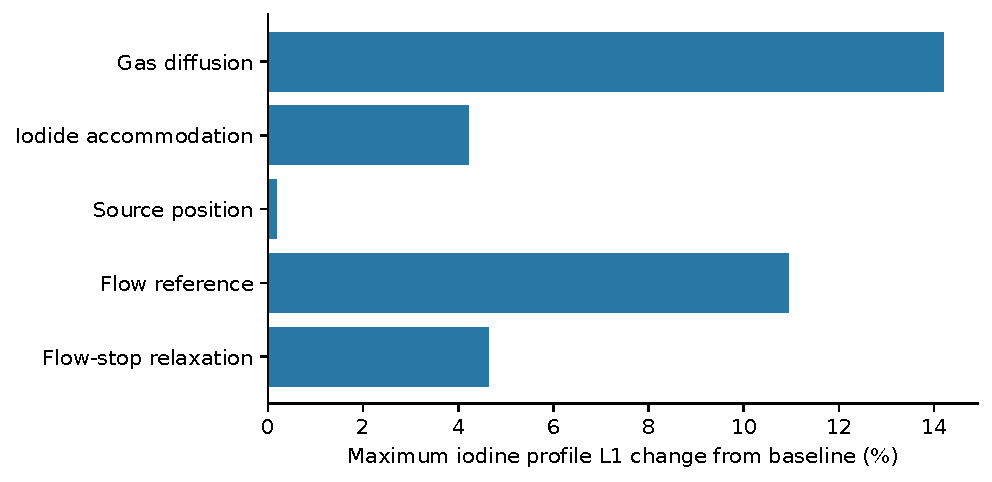
\includegraphics[width=.8\textwidth]{physical_sensitivity.pdf}
\caption{Maximum baseline-relative iodine profile changes among the
selected physical-input comparisons. Flow-stop relaxation uses an
80 s endpoint; the others use 60 s. These maxima describe the tested
case set, not a general uncertainty budget or an experimentally
identified parameter ranking.}
\label{fig:physical}
\end{figure}

\section{Conclusions}
\label{sec:conclusions}
A conservative finite-volume treatment of nine Pb--Bi--I gases and four
shared condensed wall inventories has been exercised in 15 baseline
and 64 follow-up cases. The reported calculations use a specialised
ideal-gas equilibrium kernel, a prescribed helium carrier and reversible
iodide wall exchange with half-cell diffusion resistance. Material
bookkeeping is strong: the worst raw source-driven follow-up element
residue is $8.85\times10^{-13}$ of supplied material. Conservation is
a numerical property of this model, rather than evidence that all
physical pathways have been represented.

The isolated time-step comparisons give iodine profile changes below
0.323\%, while medium-to-fine mesh comparisons give 2.06--10.58\%.
Stable total deposition and small centroid changes therefore do not
establish spatial convergence of local profiles. Closely competing
1 cm bins can also make a reported peak temperature switch by tens of
kelvin under refinement. Further spatial and full-run iteration checks
are required before claiming precise local predictive accuracy.

Thermodynamic and source assumptions materially affect the computed
iodide partition. On the refined steel case, a $+29$ kJ/mol BiI gas
Gibbs-energy surrogate changes the BiI$_3$ iodine share from 94.57\%
to 2.00\%. This sensitivity survives refinement but does not determine
which thermodynamic branch represents the experiment. Q1 agreement is
conditioned on inferred deposit masses, and Q2 retains a deposit-derived
iodine source and an unmeasured metal saturation.

For silica, input-derived temperature-coordinate shifts reduce the
original 4--5 cm position discrepancies to 0--1 cm. The improvement
identifies coordinate registration as a consequential uncertainty;
it does not establish a corrected experimental dataset. The supplied
paper does not resolve that registration or the flow-reference conditions.

The present evidence supports a methods and input-sensitivity study.
An independent predictive validation would require better-constrained
source and thermodynamic inputs, consistent experimental coordinates,
spatially qualified profile calculations and treatment of the
three-hour release and cooling protocol. The completed cases identify
where that additional evidence is needed without hiding the original
profile discrepancies.

\section*{Data and software availability}
The solver and benchmark preparation scripts are maintained in the
LESTO repository, \url{https://github.com/JanKren/LESTO}. The accompanying
working-manuscript files contain the completed baseline and follow-up
metrics, saved axial profiles, generated tables, figure-generation code
and SHA-256 provenance records. Experimental curves were digitised from
Liu et al.\ \cite{Liu2025chemical}; they are reconstructions of published
figures, rather than author-supplied measurements. Figure data are
adapted under the source paper's CC BY 4.0 licence. Some thermodynamic
coefficient files are external inputs and are not redistributed. Their
local identifiers and derived-table provenance are recorded with the
benchmark. Reproducing the CFD calculation from coefficients requires
access to those inputs; regenerating the manuscript figures uses the
saved results and does not require them.
\appendix
\section{Properties, thermodynamic provenance and units}
\label{app:properties}
\subsection{Helium and transported molecular masses}
The executed helium carrier uses
$M_{\rm He}=0.0040026\units{kg\,mol^{-1}}$,
$C_p=5193\units{J\,kg^{-1}\,K^{-1}}$ and
\begin{equation}
 \rho=\frac{pM_{\rm He}}{RT},\qquad
 \mu(T)=\frac{A_s\sqrt T}{1+T_s/T},\quad
 A_s=1.4683\times10^{-6},\quad T_s=83.40\units{K}.
\end{equation}
The numerical value of $A_s$ gives viscosity in Pa\,s when $T$ is in K.
These are case inputs to the perfect-gas, constant-heat-capacity,
Sutherland model. They are not newly fitted measured helium properties.
Pressure used in partial-pressure conversions is absolute, while
thermodynamic activities use $p^\circ=10^5\units{Pa}$. The assumed
controller reference pressure, 101,325 Pa, is a separate quantity.
\Cref{tab:masses} records the species masses used in transport and
stoichiometric conversion.
\begin{table}[tb]
\centering
\caption{Transported gas molar masses. Condensed iodide reservoirs use
the same formula masses; shared Pb and Bi inventories use atomic masses.}
\label{tab:masses}
\begin{tabular}{lr@{\qquad}lr@{\qquad}lr}
\toprule
Gas & kg/mol & Gas & kg/mol & Gas & kg/mol \\
\midrule
Pb & 0.207200 & Bi & 0.2089804 & I & 0.12690447 \\
PbI & 0.33410447 & Bi$_2$ & 0.4179608 & I$_2$ & 0.25380894 \\
PbI$_2$ & 0.46100894 & BiI & 0.33588487 & BiI$_3$ & 0.58969381 \\
\bottomrule
\end{tabular}
\end{table}

\subsection{Thermodynamic records and phase treatment}
Pb--I--He functions are evaluated from external NASA-nine-coefficient
records labelled with Gurvich source information. Bi--I functions use
an external ThermoFun compilation labelled HERACLES/Barin. The common
property evaluator converts records to a consistent absolute
$G^\circ(T)=H^\circ(T)-TS^\circ(T)$ convention before forming reaction
Gibbs energies; mixing this convention with an apparent formation-Gibbs
value would give inconsistent equilibrium constants. Tables used by the
solver store formation constants and phase-resolved vapour pressures
logarithmically. Input-file hashes, record identifiers and table-generation
scripts are recorded in the benchmark provenance.

For an iodide with one gas molecule per condensed formula unit,
\begin{equation}
 p_{\rm eq}(T)=p^\circ\exp\left[-\frac{G_g^\circ(T)
                                  -G_c^\circ(T)}{RT}\right],
 \label{eq:pv}
\end{equation}
using the stable available condensed branch. The BiI$_3$ liquid branch
is constructed at $T_{\rm fus}=680.85\units{K}$ from the crystalline
record with $\Delta H_{\rm fus}=31.798\units{kJ\,mol^{-1}}$ and
$C_{p,l}=150.624\units{J\,mol^{-1}\,K^{-1}}$, as recorded in the
input-generation metadata. It is a constructed phase record, rather
than an independently confirmed liquid thermodynamic dataset. Bi and
Bi$_2$ share condensed Bi but have different gas chemical potentials
and stoichiometry.

The BiI $+29$ kJ/mol variant alters the gas record and regenerates all
formation and disproportionation constants consistently. Baseline and
perturbed functions are hypotheses for the sensitivity calculation;
independent confirmation of the BiI source record remains needed.
External coefficient files are not reproduced in the manuscript data
package. Numerical conservation of their derived model cannot establish
their physical correctness or complete the provenance assessment.

\subsection{Optional \texorpdfstring{PbI$_2$}{PbI2}--He diffusion estimate}
Only the PbI$_2$--He transport variant uses the following implemented
correlation:
\begin{align}
 D_{\rm PbI_2-He}&=
 \frac{1.86\times10^{-7}T^{3/2}\sqrt{1/4.0026+1/461}}
 {(p/101325)\sigma^2\Omega(T^*)},\\
 T^*&=T/71.117857,\qquad \sigma=4.258468,\\
 \Omega(T^*)&=0.5313-1.2946e^{-0.9922T^*}
                     +\frac{1.5591}{T^*}-\frac{0.1918}{(T^*)^2}.
\end{align}
In this numerical expression $T$ is in K, $p$ in Pa, $\sigma$ in
\AA\ and the mass values in g/mol; the resulting $D$ is in
$\mathrm{m^2\,s^{-1}}$. The implementation retains 461 g/mol to
reproduce the original correlation, rather than the more precise
transport formula mass in \cref{tab:masses}. Its estimated collision
parameters use the original polarizability/electron-count construction
recorded in the code. Other eight gases retain the constant baseline
coefficient in this variant. The correlation is a screening alternative,
not an experimentally validated binary diffusivity or a replacement
for all missing Pb--Bi--I transport data.

\bibliographystyle{unsrtnat}
\bibliography{references}
\end{document}
